

	VxWorks系统主要如下几个组件,一般的应用程序也就用到如下几个模块:任务调度负责任务优先级,任务创建,任务删除等功能。任务通讯主要涉及队列管理,管道管理等。IO管理就是通用外设的输入输出管理。文件管理包含文件或者链接创建,修改,删除,检索等等。内存管理包含内存申请及内存释放。定时器管理就是定时器创建,定时器删除。网络通信包含套接字创建,udp/tcp通信,套接字删除,及配置管理。同步就是任务同步。互斥就是任务互斥,保护关键资源。
	
	在VxWorks操作系统的代码架构里面,一般写一个应用程序只需要涉及上面几个系统组件,由于VxWorks操作系统组件化非常好,这几个组件的耦合度非常低,每个组件对外提供都是单独的头文件,比如任务调度,其头文件为taskLib.h,任务通讯如果用的队列,那其头文件就是msgQLib.h,如果是定时器管理,那其头文件就是timerLib.h,因此也让程序移植提供了很大的便利性。有很多人认为,VxWorks跟Linux操作性的系统头文件差异化太大,因此移植难度成倍速增加,其实不然,就是由于VxWorks的高度组件化,让程序移植提供了很大的便利性。
	
	
	wind使用中断驱动和优先级的方式。它缩短了上下文转换的时间开销和中断的时间延迟。VxWorks中的任何例程都可以被启动为一个单独的任务,拥有它自己的上下文和堆栈,还有一些其他的任务机制可以使得任务挂起、继续、删除、延时或改变优先级。	
	
	
	板级支持包BSP(Board Support Package)作为VxWorks系统的主要组成部分,对各种板子的硬件功能提供了同一的软件接口,它包括硬件初始化、中断的产生和处理、硬件时钟和计时器管理、局域和总线内存地址映射、内存分配等。每一个板级支持包包括一个ROM启动(Boot ROM)或其他启动机制。



%\subsection{第二层}\label{sec:1}
%\subsubsection{第三层}\label{sec:1}
%测试测试测试测试测试测试测试测试测试测试测试测试。
%\footnote{\label{footnote:1}脚注}

\section{字体}

普通\textbf{粗体}\emph{斜体}

\hei{黑体}\kai{楷体}\fangsong{仿宋}

\section{公式}

单个公式,公式引用:\autoref{eq:1}。
\begin{equation}
 c^2 = a^2 + b^2 \label{eq:1}
\end{equation}

多个公式,公式引用:\autoref{eq:2},\autoref{eq:3}。

\begin{subequations}
\begin{equation}
  F = ma \label{eq:2}
\end{equation}
\begin{equation}
  E = mc^2 \label{eq:3}
\end{equation}
\end{subequations}

\section{罗列环境}

\begin{enumerate}
    \item 第一层\label{item:1}
    \item 第一层
    \begin{enumerate}
        \item 第二层\label{item:2}
        \item 第二层
        \begin{enumerate}
            \item 第三层\label{item:3}
            \item 第三层
        \end{enumerate}
    \end{enumerate}
\end{enumerate}

\begin{description}
    \item[解释环境]  解释内容
\end{description}



\clearpage

\section{代码环境}

\begin{lstlisting}[language=python]
import os

def main():
    '''
    doc here
    '''
    print 'hello, world' # Abc
    print 'hello, 中文' # 中文
\end{lstlisting}

\section{定律证明环境}

\begin{definition}
这是一个定义。
\end{definition}
\begin{proposition}
这是一个命题。
\end{proposition}
\begin{axiom}
这是一个公理。
\end{axiom}
\begin{lemma}
这是一个引理。
\end{lemma}

\begin{theorem}
这是一个定理。
\end{theorem}
\begin{proof}
这是一个证明。
\end{proof}

\section{算法环境}

\begin{algorithm}[H]
\SetAlgoLined
\KwData{this text}
\KwResult{how to write algorithm with \LaTeX2e }
initialization\;\label{alg_line:1}
\While{not at end of this document}{
read current\;
\eIf{understand}{
go to next section\;
current section becomes this
 one\;
}{
go back to the beginning of current section\;
}
}
\caption{How to write algorithms}\label{alg:1}
\end{algorithm}


\section{表格}
表格见\autoref{tab:1}。

\begin{table}[!h]
\centering
\caption{一个表格}\label{tab:1}
\begin{tabular}{|c|c|}
\hline
a & b \\
\hline
c & d \\
\hline
\end{tabular}
\end{table}
\section{图片}
图片见\autoref{fig:1}。图片格式支持eps,png,pdf等。多个图片见\autoref{fig:2},分开引用:\autoref{fig:2-1},\autoref{fig:2-2}。

\begin{figure}[!h]
\centering

\includegraphics[width=.4\textwidth]{hust-title.pdf}
\caption{hust-title}\label{fig:hust-title}
\end{figure}

\begin{figure}[!h]
\centering
  \begin{subfigure}[b]{0.3\textwidth}
  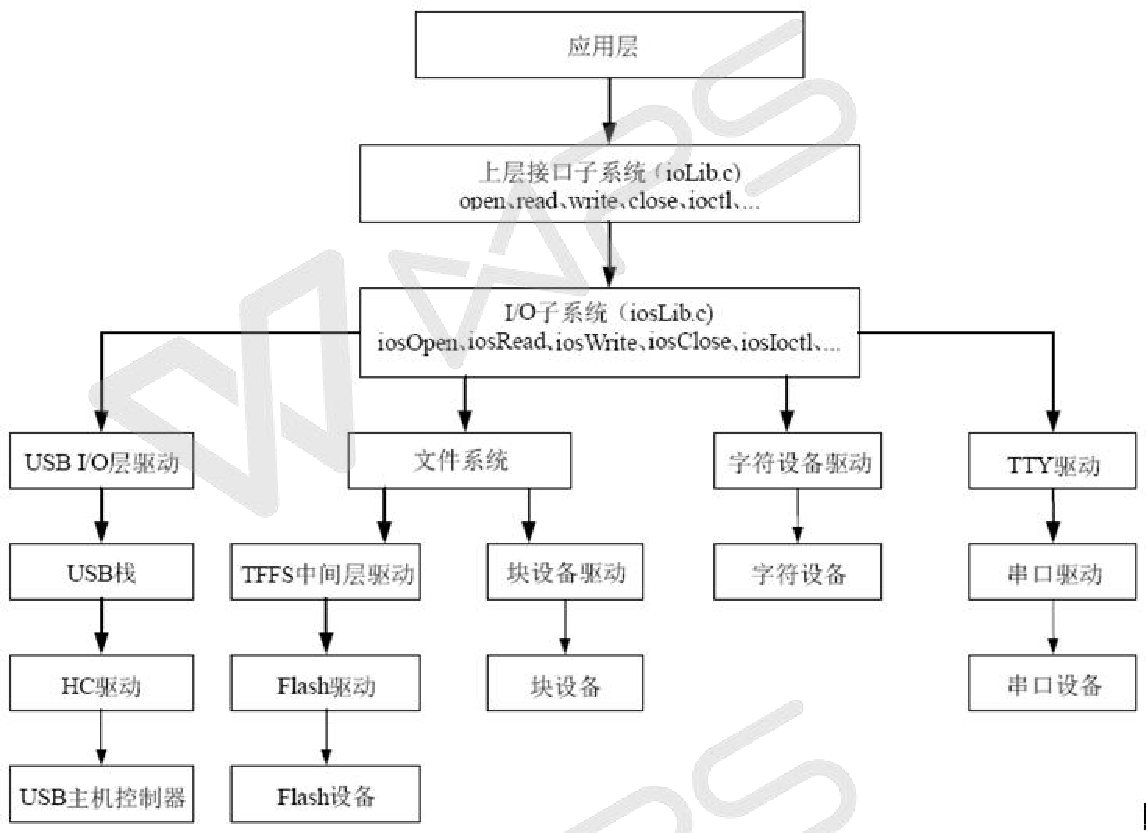
\includegraphics[width=\textwidth]{./graphics/VxWorks-driver-structure.pdf}
  \caption{VxWorks-driver-structure}
  \end{subfigure}
  ~
  \begin{subfigure}[b]{0.3\textwidth}
  \includegraphics[width=\textwidth]{}
  \caption{图片2}\label{fig:2-2}
  \end{subfigure}
\caption{多个图片}\label{fig:2}
\end{figure}

\section{参考文献示例}
这是一篇中文参考文献\cite{徐媛媛2003嵌入式实时操作系统的设备驱动};这是一篇英文参考文献\cite{9787508342894};同时引用\cite{9780124467422,bamboosilk}。

\section[\textbackslash{}autoref 测试]{\texttt{\textbackslash{}autoref} 测试}

\begin{description}
  \item[公式] \autoref{eq:1}
  \item[脚注] \autoref{footnote:1}
  \item[项] \autoref{item:1},\autoref{item:2},\autoref{item:3}
  \item[图] \autoref{fig:1}
  \item[表] \autoref{tab:1}
  \item[附录] \autoref{appendix:1}
  \item[章] \autoref{chapter:1}
  \item[小节] \autoref{sec:1},\autoref{sec:2},\autoref{sec:3}
  \item[算法] \autoref{alg:1},\autoref{alg_line:1}
  \item[证明环境] \autoref{def:1},\autoref{proposition:1},\autoref{axiom:1},\autoref{lemma:1},\autoref{theorem:1},\autoref{proof:1}
\end{description}